\documentclass[UTF8]{article}

%--
\usepackage{ctex}
\usepackage[margin=1in]{geometry}
\usepackage{amsmath}
\usepackage{mathrsfs}
\usepackage{graphicx}
\usepackage{caption,subcaption}

%--
\begin{document}
    
%--
{\flushleft \bf \Large 姓名:} 李青坪

{\flushleft \bf \Large 学号:} MF1733034

{\flushleft \bf \Large 日期:} 2017.11.16


%=========================================================================
\section*{论文信息}
    
Özalp Babaoğlu, Fromentin E, Raynal M. A unified framework for the specification and run-time detection of dynamic properties in distributed computations ☆[M]. Elsevier Science Inc. 1996.

    
%=========================================================================
\section{简介}

复杂的分布式程序的可靠性依赖于有效测试和调试分布式程序的执行的能力。因此需要我们具有规约分布式计算中所涉及的动态属性的能力,以及构造一个算法在运行时检测这些动态属性的能力。通俗地说,动态属性是指一个分布式程序的状态的时间演变,动态属性定义了程序执行过程中的一些执行序列的子集。本文是把动态属性的规约和检测问题形式化为语言检测问题。考虑计算状态的布尔谓词作为字母表,动态属性规约就好比在这张字母表上定义语言,而动态属性检测类似于在运行时检测一个分布式计算产生的句子是否属于该语言。

分布式程序有三个时间段可以用来验证属性:执行前、执行中和执行后,在执行前验证属性就需要我们描述程序所有可能的执行,模型检测技术就是在执行前验证属性的技术,利用状态迁移系统(S)表示系统的行为,用模态逻辑公式(F)描述系统的性质,判断状态迁移系统S是否是公式F的一个模型,即可判断系统是否具有某种性质。运行时验证的方法是看程序执行的一个观测结果是否满足属性而不是从程序所有可能的执行中得出结论。执行后验证基于执行时收集的数据,需要在执行完后验证,对很多应用程序不适用。

本文要考虑的问题是规约不稳定的属性以及在运行时检测这些属性。不稳定属性,顾名思义,是指在程序执行过程中不断改变的属性,本文根据形式化语言理论设计了属性规约以及检测的框架。该框架是基于一个有向无环图(DAG)的标签,DAG中的每个结点都关联一组属于给定字母表中标签,每条路径也都是关联从相同的字母表中构建的一组单词,与终止于一个节点的所有路径相对应的所有单词的集合就定义了一种语言。本文在第三章描述了一个通用的属性规约和检测的框架,并在第四章和第五章分别基于局部状态的DAG和全局状态的格的DAG实例化了该框架。

\section{分布式计算}
分布式计算是由一组通过交换信息实现通信的进程的执行实现的,进程既不能访问共享内存也不能访问全局时钟。分布式计算可以分为三类:

\begin{itemize}
	\item 作为偏序集的分布式计算:用H表示所有事件的集合,$\rightarrow$表示事件之间因果优先关系的二元关系,$ e_i^a $表示进程$ P_i $的第a个事件。定义事件的因果优先关系如下:
	\begin{align}
	e_i^a \rightarrow e_j^b \equiv \left\{
	\begin{aligned}
		&(i=j)\land(b=a+1) \quad  or\\
		&(e_i^a=send(m))\land (e_j^b=receive(m)) \quad  or \\
		&\exists e_k^c:(e_i^a \rightarrow e_k^c)\land (e_k^c \rightarrow e_j^b).
	\end{aligned}
	\right.
	\end{align}
	则一个分布式计算可以被建模为一个偏序集$ \mathscr{H}=(H,\rightarrow) $,表示分布式计算的事件执行序列的偏序,对于没有因果优先关系的事件,我们无法给出它们执行的先后顺序,所以不能得到分布式计算中事件执行的全序,只能用偏序集表示。
	\item 作为局部状态的有向无环图的分布式计算:用S表示所有局部状态的集合,$ \prec $表示状态之间的立即因果优先关系,$ \sigma_i^a $表示进程$ P_i $执行完$ e_i^a $之后的局部状态。定义局部状态的因果优先关系如下:
	\begin{align}
	\sigma_i^a \prec \sigma_j^b \equiv \left\{
	\begin{aligned}
		&(i=j)\land(b=a+1) \quad  or\\
		&(e_i^{a+1}=send(m))\land (e_j^b=receive(m)) \\
	\end{aligned}
	\right.
	\end{align}
	注意式(2)的第二个条件是$ e_i^{a+1}=send(m))\land (e_j^b=receive(m)) $,前面是$ e_i^{a+1} $,表示在$ e_i^{a+1} $执行之后达到的状态与$ \sigma_j^b $之间并没有因果优先关系,$ \sigma_j^b $只与$ \sigma_j^a $有因果优先关系。则一个分布式计算可以被建模为一个DAG:$ \mathscr{S} = (S,\prec)$
	\item 作为全局状态格的分布式计算:全局状态$ \Sigma = (\sigma_1,\sigma_2,...,\sigma_n) $是局部状态的n元组,每个局部状态对应一个进程的局部状态,且该全局状态$ \Sigma $内部的局部状态之间都是没有因果优先关系的,否则该全局状态是不可能达到的。用$ \mathscr{L} $表示格,$ \Sigma = (\sigma_1,...,\sigma_i^a,...,\sigma_n) $到$ \Sigma = (\sigma_1,...,\sigma_i^{a+1},...,\sigma_n) $存在边,当且仅当在局部状态$ \sigma_i^a $下,存在事件e可被$ P_i $执行,使$ P_i $到达$ \sigma_i^{a+1} $状态。
\end{itemize}

\section{通用框架}
该框架基于一个有向无环图G和一个有限的标签字母表A,G中的每个结点都由一组属于A中的标签标记,从初始结点开始到结点v结束的一组结点序列构成一条有向边(即路径),由该路径上的所有结点的标签按执行顺序构造的单词集叫做路径标签,记为$ \tilde{\lambda}(\pi_v) $,所有到达v的路径标签的集合便可视为构造了语言$ L^{\lambda}(v) $。在字母表A上定义一组单词集,表示动态属性,只要$ L^{\lambda}(v) $中存在一个与$ L(\Phi) $中定义的单词相同的单词,则$ v \models \textbf{SOME} \ \Phi $;如果$ L^{\lambda}(v) $是$ L(\Phi) $的子集,则$ v \models \textbf{ALL} \ \Phi $。

本文设计动态属性时,使动态属性满足正则语法,$ L(\Phi) $表示一种正则语言,定义了一组可接收的状态$ Q_F $。在执行了$ L^{\lambda}(v) $中所有的单词后,有限自动机根据$ L(\Phi) $定义的语言产生结果状态集,用$ R^{\Phi}(v) $表示,$ R^{\Phi}(v) $可以通过文章中图6给出的算法求解。对有向无环图G中的每个结点v计算$ R^{\Phi}(v) $,就完成了动态属性的检测。根据可接收状态与自动机可达到的状态之间的关系表述满足规则:
$$
\begin{aligned}
	&v \models \textbf{SOME} \ \Phi \equiv (R^{\Phi}(v) \cap Q_F \neq \emptyset) \\
	&v \models \textbf{ALL} \ \Phi \equiv (R^{\Phi}(v) \subseteq Q_F).
\end{aligned}
$$

如果在使用该通用框架时,关注的是局部状态的序列,则将该框架应用于控制流上的属性检测。这里的字母表将由局部谓词(即布尔表达式)组成。根据该字母表,我们可以定义局部状态的行为模式,即在计算时需要按特定顺序被满足的、由一组谓词指定的属性类别。给定局部谓词的字母表,与局部状态的控制流相关联的语言$ L(\Phi) $可以表达属性$ \Phi $所允许的行为模式。满足规则依然有两条:
$$
\begin{aligned}
	&\sigma \models \textbf{SOME} \ \Phi \equiv (L^{\lambda}(\sigma) \cap L(\Phi) \neq \emptyset) \\
	&\sigma \models \textbf{ALL} \ \Phi \equiv (L^{\lambda}(\sigma) \subseteq L(\Phi)).
\end{aligned}
$$
进行动态属性检测时,可以按照图6所示的算法进行,只需要额外维护一个数组$ B_i[Q] $。$ B_i[q]=true $,当且仅当存在一条终止于$ P_i $的当前局部状态$ \sigma $的控制流,使得$ \tilde{\lambda}(\pi_{\sigma}) $中至少有一个单词使自动机达到状态q。执行图8中的算法即可计算$ B_i[Q] $,通过$ B_i[Q] $即可完成动态属性检测,满足规则有以下两条:
$$
\begin{aligned}
	&\sigma \models \textbf{SOME} \ \Phi \equiv \exists q\in Q:((B_{\sigma}[q]=true) \land q \in Q_F) \\
	&\sigma \models \textbf{ALL} \ \Phi \equiv \forall q\in Q:((B_{\sigma}[q]=true) \Rightarrow q \in Q_F).
\end{aligned}
$$

\begin{figure}[htbp]
\centering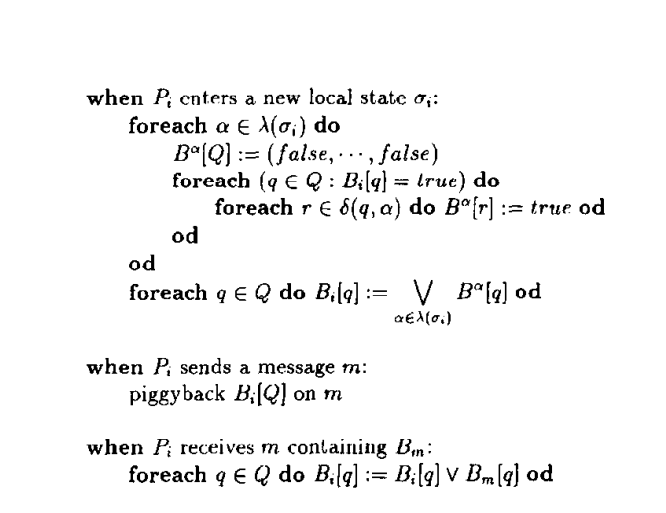
\includegraphics[width=5in]{fig8.png}
\caption*{图8:进程$ P_i $的控制器为了在控制流上检测属性而执行的算法}
\label{fig:8}
\end{figure}
如果在使用通用框架时,关注的是全局状态的序列,则将该框架应用于基于观测的属性检测。在实现动态属性检测时与控制流上的属性检测类似,不同之处是这里使用一个监视器来构造格和检查属性,并通过该监视器收集进程的局部状态来维护全局状态的一致性。

\section{主要贡献}
本文提出了分布式计算的模型,即作为偏序集的分布式计算、作为局部状态的有向无环图的分布式计算和作为全局状态格的分布式计算,构造了规约和检测动态属性的统一框架并提出基于控制流和观测的属性检测算法。如果谓词是定义在局部状态上,则行为模式是在计算的控制流上;如果谓词是定义在全局状态上,则行为模式是在计算的观测上。本文在一个分布式调试设备EREBUS上实现了动态属性检测,但只实现了在控制流上检测动态属性。基于观测的属性检测工作最大的问题是格的构造,因为构造的时候很容易造成指数爆炸,使得基于观测的属性检测显得不太可行。

本文提出的分布式计算模型假设进程间的通信是可靠的,即不考虑进程通信时可能出现的消息丢失。虽然消息丢失出现的概率很小,但是如果在网络环境较差的情况下,为了保证动态属性检测的正确性,我们还是需要考虑进程间通信的可靠性。比如在控制流上进行属性检测时,执行图8中的算法,需要将$ B_m $封装在消息中发送给其他进程,这时$ B_m $如果出错或者丢失的话,将会影响属性检测的结果,某些属性可能无法检测出来。另外,对于属性的检测最好做成启发式的,程序执行的过程中变量、环境都在不断的变化,属性检测算法应该能较快速地构造路径标签。对于基于观测的属性检测来说,就是避免格的构造带来的指数爆炸,不要求算法能给出解空间中的每一个解,只需要根据经验得到接近最优解的一组可行解即可。

    
%--
\end{document}